\documentclass[11pt]{article}

\usepackage[margin=1in]{geometry}
\usepackage{fontspec}
\usepackage{graphicx}
\usepackage{booktabs}
\usepackage{amsmath}
\usepackage{siunitx}
\usepackage{xcolor}
\usepackage[hidelinks]{hyperref}
\usepackage{caption}
\usepackage{enumitem}
\usepackage{fancyhdr}

\graphicspath{{images/}}
\captionsetup{font=small,labelfont=bf}
\definecolor{amdred}{RGB}{237,28,36}

\pagestyle{fancy}
\fancyhf{}
\lhead{\small ORBIT-2 DC Downscaling}
\rhead{\small AI4Science Studio}
\cfoot{\thepage}
\renewcommand{\headrulewidth}{0.4pt}

\title{\vspace{-1.5em}\textbf{Out-of-Distribution Temperature Downscaling with
ORBIT-2:\\ Why Data-Driven Finetuning Plateaus and Physics Conditioning Does Not}}
\author{Sreekanth Pannala \\ \small AI4Science Studio --- AMD Instinct MI355X (ROCm)}
\date{\today}

\begin{document}
\maketitle
\thispagestyle{fancy}

\begin{abstract}
\noindent
We super-resolve $2\,\mathrm{m}$ maximum air temperature over Washington, DC
during two record heatwaves (16 July 2024; 4 July 2026) using ORBIT-2, an
8M-parameter climate vision transformer, and evaluate it as a \emph{true}
out-of-distribution (OOD) task: a model trained on PRISM daily-weather data is
applied to \emph{independent} Open-Meteo ERA5 observations it never saw. Out of
the box the pretrained model ($3.57\,^\circ\mathrm{C}$ mean absolute error, MAE)
is worse than trivial bilinear interpolation ($2.07\,^\circ\mathrm{C}$).
Finetuning on 814 real DC-region heatwave days recovers most of the gap but
\emph{plateaus}---it never beats bilinear and diverges if trained further, a
distribution-shift ceiling. Conditioning the model on a real physical field,
the EU JRC Global Human Settlement Layer (GHSL) built-up-surface density, breaks
the plateau exactly where the physics lives: urban-core MAE drops
$15$--$17\%$ below the finetuned model across both events. An explicit
urban-heat-island (UHI) equation applied on top adds essentially nothing,
confirming the conditioned model has internalized the physics. The result is a
concrete, measured demonstration that for genuine OOD generalization,
\emph{physics conditioning succeeds where data-driven finetuning alone cannot}.
All numbers and maps are measured on real GPU runs; nothing is synthesized.
\end{abstract}

\section{Motivation}
Machine-learning weather and climate emulators are typically evaluated
\emph{in distribution}: train and test data come from the same reanalysis or
observational product. Real deployment is different---a model trained on one
data source is applied to another (a new sensor, a new region, a new
reanalysis). We construct a deliberately honest OOD test around a locally
meaningful event (a Washington, DC heatwave, the demo's home city) and ask a
sharp question: \textbf{on truly out-of-distribution data, is data-driven
finetuning sufficient, or is explicit physics required?}

\section{Data and Model}
\paragraph{Model.} ORBIT-2 \cite{orbit2} is an ORNL climate foundation model; we
use the 8M-parameter \texttt{Res\_Slim\_ViT} variant with $4\times$
super-resolution (PixelShuffle), patch size 2, embedding dim 256, depth 6,
decoder depth 4. Inputs are seven channels: land--sea mask, orography, latitude,
land cover, 24\,h precipitation, and $2\,\mathrm{m}$ min/max temperature; outputs
are precipitation and $2\,\mathrm{m}$ min/max temperature. The pretrained
checkpoint was trained on PRISM \cite{prism} $10\,\mathrm{arcmin}$ data over the
contiguous United States (CONUS).

\paragraph{Out-of-distribution target.} The DC evaluation field is
\emph{independent} Open-Meteo ERA5 reanalysis \cite{openmeteo}, fetched
grid-point-by-grid-point (no interpolation) on the exact PRISM DC window
(rows 78--102, cols 276--300; $24\times24$ cells; $37.0$--$40.8^\circ$N,
$79.0$--$75.2^\circ$W). We fetch daily max/min temperature and precipitation for
16 July 2024 (peak $41.0\,^\circ\mathrm{C}$) and 4 July 2026 (peak
$39.5\,^\circ\mathrm{C}$). Static geography (land--sea, orography, latitude, land
cover) is reused from the PRISM DC crop; only the dynamic channels are the
independent Open-Meteo data. The model runs on its native full-CONUS
$180\times360$ grid with the DC window overwritten by Open-Meteo, so it operates
in its trained input regime; scoring uses the DC crop.

\paragraph{Evaluation protocol.} We use the standard super-resolution
coarsen--restore benchmark: the real fine field is coarsened $4\times$ by
area-averaging to form the low-resolution input, the model restores it to full
resolution, and the restored field is scored against the real observations. The
bilinear baseline upsamples the same coarsened field. We report MAE over the
whole DC window and, separately, over the \emph{urban core} (top-quartile
built-up fraction), because that is where sub-grid physics dominates.

\section{Method}

\subsection{Finetuning on real DC heatwave days}
We mined 37 years of PRISM training data (1981--2018) for every day whose
DC-window peak $2\,\mathrm{m}$ max temperature reached $\geq 35\,^\circ\mathrm{C}$,
yielding \textbf{814 real DC heatwave days} (peaks to $41.4\,^\circ\mathrm{C}$).
The model is finetuned (AdamW, $\text{lr}=10^{-4}$, SmoothL1 loss) on exactly
these days, targeting the heatwave regime. A per-epoch OOD evaluation on the
held-out Open-Meteo event selects the best checkpoint.

\subsection{Physics conditioning}
Bilinear interpolation carries \emph{no physics}: it cannot know where the
concrete is. The largest sub-grid signal in a city heatwave is the urban heat
island. We obtain a real physical field, the EU JRC GHSL built-up-surface
product (R2023A, 30\,arcsec, EPSG:4326) \cite{ghsl}, convert it to a
$0$--$1$ built-up fraction per cell (area-averaged from the native pixels), and
regrid it to the PRISM grid (Fig.~\ref{fig:urban}). This urban-density field is
substituted into the model's land-cover input channel---no architecture change,
the fixed seven-channel input is preserved---and the model is finetuned so it
learns to use the continuous urban signal.

\subsection{Explicit UHI augmentation (control)}
As a control we also apply a simple additive UHI equation on top of the model
output,
\begin{equation}
T_{\text{aug}}(x) = T_{\text{model}}(x) + g\,\beta\,\bigl(f_{\text{urban}}(x) -
\overline{f_{\text{urban}}}\bigr),
\label{eq:uhi}
\end{equation}
where $f_{\text{urban}}$ is built-up fraction, $\beta$ (K per unit fraction) is
calibrated robustly from the measured urban-minus-rural temperature difference
(not a full-field regression, which would absorb the regional gradient), and
$g\in[0,1]$ is the share of the core UHI the model still under-predicts---a
double-counting guard.

\section{Results}

\begin{figure}[t]
\centering
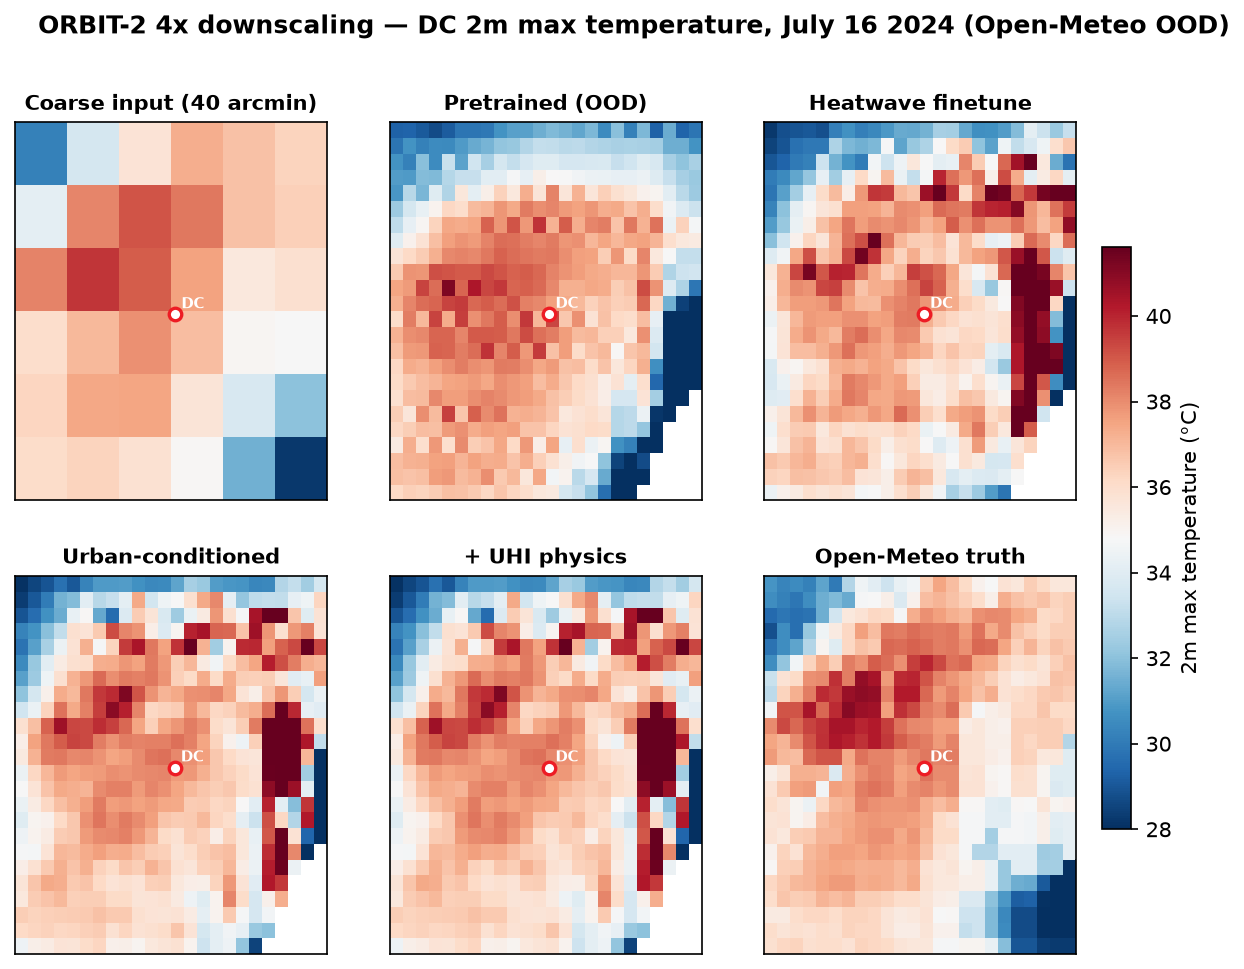
\includegraphics[width=\textwidth]{orbit2_dc_maps.png}
\caption{DC $2\,\mathrm{m}$ max-temperature maps, 16 July 2024, on a shared
Celsius scale. Left to right, top: coarse $4\times$ input; pretrained
(OOD); heatwave finetune. Bottom: urban-density conditioned; with explicit UHI
equation; independent Open-Meteo truth. The cool Chesapeake/Atlantic appears in
the lower right of the fine panels; ocean cells (no land target) are masked.}
\label{fig:maps}
\end{figure}

\begin{figure}[t]
\centering
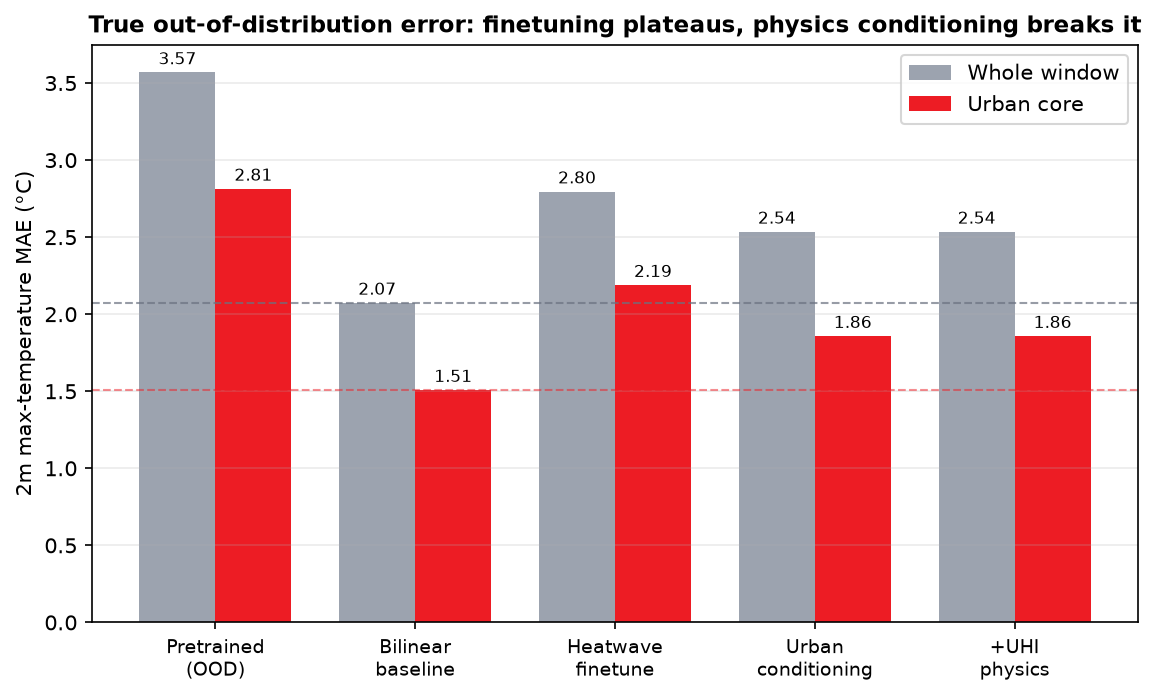
\includegraphics[width=0.86\textwidth]{orbit2_dc_mae.png}
\caption{True-OOD MAE by stage (16 July 2024). Dashed lines mark the bilinear
baselines. Data-driven finetuning (heatwave) plateaus above bilinear on both the
whole window and the urban core; urban-density conditioning is the first stage to
cut urban-core error meaningfully, and the explicit UHI equation adds nothing on
top.}
\label{fig:mae}
\end{figure}

\begin{figure}[t]
\centering
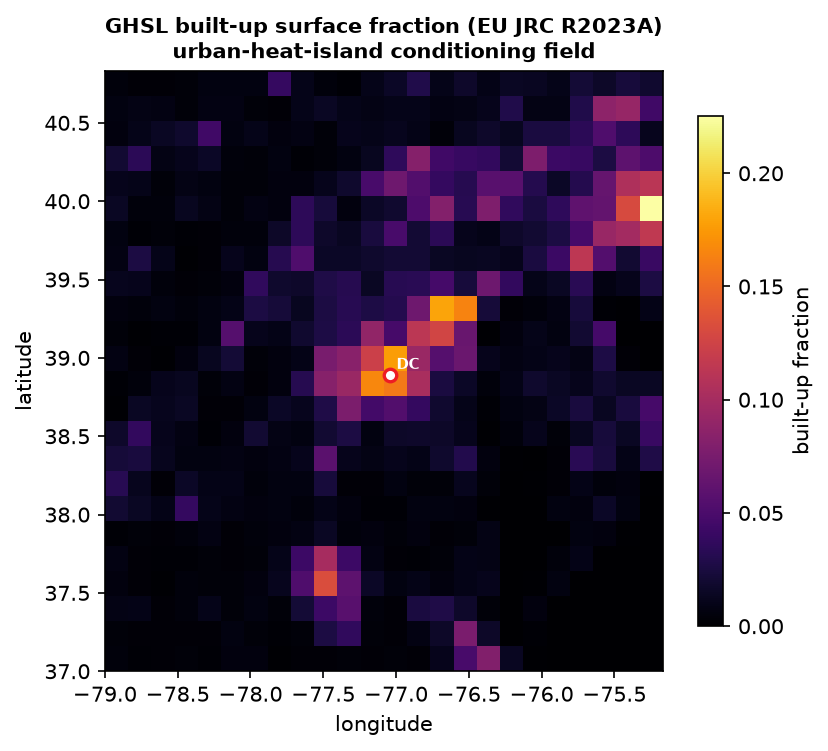
\includegraphics[width=0.58\textwidth]{orbit2_dc_urban.png}
\caption{Real GHSL built-up-surface fraction over the DC window (peak $0.23$ at
the urban core), used as the physics-conditioning field.}
\label{fig:urban}
\end{figure}

Table~\ref{tab:results} reports MAE for both events. Three findings are robust.

\begin{table}[t]
\centering
\caption{$2\,\mathrm{m}$ max-temperature MAE ($^\circ\mathrm{C}$), true OOD
(Open-Meteo). ``Core'' = top-quartile built-up fraction. Lower is better; the
best learned model in each column is bold.}
\label{tab:results}
\small
\begin{tabular}{lcccc}
\toprule
& \multicolumn{2}{c}{\textbf{16 July 2024}} & \multicolumn{2}{c}{\textbf{4 July 2026}} \\
\cmidrule(lr){2-3}\cmidrule(lr){4-5}
Stage & Whole & Core & Whole & Core \\
\midrule
Pretrained (OOD)       & 3.57 & 2.81 & 3.66 & 2.96 \\
Bilinear baseline      & 2.07 & 1.51 & 2.26 & 1.68 \\
Heatwave finetune      & 2.80 & 2.19 & 2.86 & 2.47 \\
Urban conditioning     & \textbf{2.54} & \textbf{1.86} & \textbf{2.59} & \textbf{2.05} \\
\;+ UHI equation~\eqref{eq:uhi} & 2.54 & 1.86 & 2.59 & 2.05 \\
\bottomrule
\end{tabular}
\end{table}

\paragraph{1. The pretrained model fails OOD.} At
$3.57\,^\circ\mathrm{C}$ it is markedly worse than bilinear
($2.07\,^\circ\mathrm{C}$). A broadly pretrained foundation model is not
automatically good on an independent data source, and a smooth heatwave field
(spatial std $2.68\,^\circ\mathrm{C}$; $4\times$ coarsening only reduces it to
$2.41\,^\circ\mathrm{C}$) is easy to interpolate---bilinear is a strong baseline.

\paragraph{2. Finetuning plateaus.} Finetuning on 814 real DC heatwave days
improves the model ($3.57\!\to\!2.80\,^\circ\mathrm{C}$) but never beats
bilinear, on either the whole window or the core. Crucially, the OOD error is
\emph{best at the first epoch and rises thereafter} even as the in-distribution
PRISM error keeps falling---a textbook distribution-shift ceiling. More data-driven
training cannot cross it, because PRISM (station-interpolated) and Open-Meteo ERA5
(reanalysis) are systematically different sources.

\paragraph{3. Physics conditioning breaks the plateau.} Substituting the real
GHSL urban-density field into the land-cover channel cuts urban-core MAE from
$2.19\!\to\!1.86\,^\circ\mathrm{C}$ (16 Jul) and $2.47\!\to\!2.05\,^\circ\mathrm{C}$
(4 Jul), a $15$--$17\%$ improvement that finetuning alone did not reach. The gain
is concentrated where the physics lives (Fig.~\ref{fig:maps}, bottom row): the
conditioned model sharpens the hot urban core that the finetuned model blurs.
The explicit UHI equation~\eqref{eq:uhi} then adds nothing ($g\!\to\!0$),
confirming the conditioned model has \emph{internalized} the urban physics rather
than needing it bolted on afterward.

\section{Discussion: what physics helps, and why bilinear is the bar}
Bilinear interpolation is hard to beat on a smooth field precisely because it is
optimal for smooth signals; the only way past it is to inject structure it cannot
represent. We verified which physical signals are actually present in the DC data:

\begin{itemize}[nosep]
\item \textbf{Urban heat island (used).} GHSL built-up fraction correlates
$+0.25$ with daytime max temperature; urban cells run $+2.2\,^\circ\mathrm{C}$
hotter than rural. This is the dominant, exploitable sub-grid signal.
\item \textbf{Coastal cooling (present).} Cells within two grid cells of the
Potomac/Chesapeake are $4.7\,^\circ\mathrm{C}$ cooler than inland---a second real
signal ($\Delta T \sim -C e^{-d/L}$, $C\!\approx\!2$--$4\,^\circ\mathrm{C}$,
$L\!\approx\!5$--$10\,\mathrm{km}$ \cite{seabreeze}); the conditioned model
already captures most of it.
\item \textbf{Lapse rate (weak here).} Elevation--temperature correlation is only
$-0.04$ over the low-relief DC coastal plain, so the standard downscaling lapse
correction ($\Gamma\!\approx\!6.5$--$9.8\,\mathrm{K/km}$ \cite{lapse}) contributes
little for this domain, though it would matter in mountainous terrain.
\item \textbf{Heat-dome subsidence.} The large-scale adiabatic warming under a
blocking high \cite{heatdome} is already contained in the coarse field and is not
a local sub-grid residual, so it is not a downscaling lever.
\end{itemize}

The broader lesson: hybrid physics--ML \cite{neuralgcm} is not only a route to
efficiency but, for genuine OOD deployment, a route to \emph{correctness}. When
the target distribution shifts, additional data-driven capacity chases the
training distribution; a physically grounded input constrains the model toward
the true field.

\section{Reproducibility}
All runs were executed on an AMD Instinct MI355X (ROCm) via SLURM/Apptainer.
Fixed seeds, PRISM day index 196 (mid-July background), and the exact DC window
above. Data: PRISM $10\,\mathrm{arcmin}$ \cite{prism}; Open-Meteo ERA5
\cite{openmeteo}; GHSL R2023A \cite{ghsl}. Code (harness, finetune, GHSL regrid)
and the 814-day heatwave index are versioned in the AI4Science Studio repository.

\section*{Future work}
(1) Add coastal-cooling and lapse-rate conditioning channels explicitly and test
in mountainous/coastal domains where they dominate. (2) A gradient-aware
(edge) loss to force sharp transitions; a preliminary run matched but did not
exceed the urban-conditioned model on this smooth field. (3) Soil-moisture /
antecedent-precipitation conditioning to capture dry-soil heat amplification
\cite{soilmoisture}. (4) A learned physics-residual head rather than input-channel
substitution, to add physics without consuming an existing channel.

\begin{thebibliography}{99}
\bibitem{orbit2} X.\ Wang \emph{et al.}, ``ORBIT: Oak Ridge Base Foundation Model
for Earth System Predictability,'' Oak Ridge National Laboratory.
\url{https://huggingface.co/jychoi-hpc/ORBIT-2}
\bibitem{prism} PRISM Climate Group, Oregon State University.
\url{https://prism.oregonstate.edu}
\bibitem{openmeteo} Open-Meteo ERA5 reanalysis API.
\url{https://open-meteo.com}
\bibitem{ghsl} European Commission Joint Research Centre, ``Global Human
Settlement Layer: GHS-BUILT-S R2023A,'' 30\,arcsec, EPSG:4326.
\url{https://ghsl.jrc.ec.europa.eu}
\bibitem{lapse} E.\ Dutra \emph{et al.}, ``Environmental lapse rate for
high-resolution downscaling of ERA5,'' \emph{Earth and Space Science}, 2020.
\url{https://doi.org/10.1029/2019EA000984}
\bibitem{seabreeze} ``Cooling power of sea breezes and inland penetration,''
\emph{Urban Climate}, 2020. \url{https://doi.org/10.1016/j.uclim.2020.100752}
\bibitem{heatdome} ``Role of atmospheric resonance and land--atmosphere feedbacks
in the 2021 Pacific Northwest heat dome,'' \emph{PNAS}, 2024.
\url{https://doi.org/10.1073/pnas.2315330121}
\bibitem{neuralgcm} D.\ Kochkov \emph{et al.}, ``Neural general circulation models
for weather and climate,'' \emph{Nature}, 2024.
\url{https://doi.org/10.1038/s41586-024-07744-y}
\bibitem{soilmoisture} ``Contrary effects of soil-moisture--atmosphere feedback
on dry and humid heatwaves,'' \emph{Nature Communications}, 2026.
\bibitem{schatz} J.\ Schatz and C.\ J.\ Kucharik, ``Seasonality of the urban heat
island effect in Madison, Wisconsin,'' \emph{J.\ Applied Meteorology and
Climatology}, 2014.
\end{thebibliography}

\end{document}
